\documentclass[11pt]{article}           
\usepackage[UTF8]{ctex}
\usepackage[a4paper]{geometry}
\geometry{left=2.0cm,right=2.0cm,top=2.5cm,bottom=2.25cm}

\usepackage{xcolor}
\usepackage{paralist}
\usepackage{enumitem}
\setenumerate[1]{itemsep=1pt,partopsep=0pt,parsep=0pt,topsep=0pt}
\setitemize[1]{itemsep=0pt,partopsep=0pt,parsep=0pt,topsep=0pt}
\usepackage{comment}
\usepackage{booktabs}
\usepackage{graphicx}
\usepackage{float}
\usepackage{sgame} % For Game Theory Matrices 
% \usepackage{diagbox} % Conflict with sgame
\usepackage{amsmath,amsfonts,graphicx,amssymb,bm,amsthm}
%\usepackage{algorithm,algorithmicx}
\usepackage{algorithm,algorithmicx}
\usepackage[noend]{algpseudocode}
\usepackage{fancyhdr}
\usepackage{tikz}
\usepackage{pgfplots}
\pgfplotsset{compat=1.18}
\usepackage{graphicx}
\usetikzlibrary{arrows,automata}
\usepackage[hidelinks,colorlinks, citecolor=blue]{hyperref}
\usepackage{extarrows}
\usepackage{totcount}
\setlength{\headheight}{14pt}
\setlength{\parindent}{0 in}
\setlength{\parskip}{0.5 em}
\usepackage{helvet}
\usepackage{dsfont}
% \usepackage{newtxmath}
\usepackage[labelfont=bf]{caption}
\renewcommand{\figurename}{Figure}
\usepackage{lastpage}
\usepackage{istgame}
\usepackage{cleveref}
\crefname{figure}{\textbf{Figure}}{Figures}
\crefname{table}{\textbf{Table}}{Tables}
\usepackage{tcolorbox}
\usepackage{minted}

\renewcommand{\tablename}{Table}

\definecolor{LightGray}{gray}{0.9}
\setminted{autogobble = true, baselinestretch = 0.9, beameroverlays = on, escapeinside=||}

% \setlength\partopsep{0pt}
% \setlength\topsep{0pt}
\setlength\parskip{0pt}
% \setlength\itemsep{0pt}
% \setlength\parsep{0pt}
% \setlength{\belowcaptionskip}{0pt}
% \setlength{\abovecaptionskip}{0pt}
% \setlength{\intextsep}{0pt}
% \setlength{\textfloatsep}{0pt}
% \setlength{\floatsep}{0pt}

% \newdateformat{mydate}{\shortmonthname[\THEMONTH]. \THEDAY \THEYEAR}

\RequirePackage{algorithm}

\makeatletter
\newenvironment{algo}
  {% \begin{breakablealgorithm}
    \begin{center}
      \refstepcounter{algorithm}% New algorithm
      \hrule height.8pt depth0pt \kern2pt% \@fs@pre for \@fs@ruled
      \parskip 0pt
      \renewcommand{\caption}[2][\relax]{% Make a new \caption
        {\raggedright\textbf{\fname@algorithm~\thealgorithm} ##2\par}%
        \ifx\relax##1\relax % #1 is \relax
          \addcontentsline{loa}{algorithm}{\protect\numberline{\thealgorithm}##2}%
        \else % #1 is not \relax
          \addcontentsline{loa}{algorithm}{\protect\numberline{\thealgorithm}##1}%
        \fi
        \kern2pt\hrule\kern2pt
     }
  }
  {% \end{breakablealgorithm}
     \kern2pt\hrule\relax% \@fs@post for \@fs@ruled
   \end{center}
  }
\makeatother


\newtheorem{theorem}{Theorem}
\newtheorem{lemma}[theorem]{Lemma}
\newtheorem{proposition}[theorem]{Proposition}
\newtheorem{claim}[theorem]{Claim}
\newtheorem{corollary}[theorem]{Corollary}
\newtheorem{definition}[theorem]{Definition}
\newtheorem*{definition*}{Definition}

\newenvironment{problem}[2][Problem]{\begin{trivlist}
    \item[\hskip \labelsep {\bfseries #1}\hskip \labelsep {\bfseries #2.}]\songti}{\hfill$\blacktriangleleft$\end{trivlist}}
\newenvironment{answer}[1][Solution]{\begin{trivlist}
    \item[\hskip \labelsep {\bfseries #1.}\hskip \labelsep]}{\hfill$\lhd$\end{trivlist}}

\newcommand\1{\mathds{1}}
% \newcommand\1{\mathbf{1}}
\newcommand\R{\mathbb{R}}
\newcommand\E{\mathbb{E}}
\newcommand\N{\mathbb{N}}
\newcommand\NN{\mathcal{N}}
\newcommand\per{\mathrm{per}}
\newcommand\PP{\mathbb{P}}
\newcommand\dd{\mathrm{d}}
\newcommand\ReLU{\mathrm{ReLU}}
\newcommand{\Exp}{\mathrm{Exp}}
\newcommand{\arrp}{\xrightarrow{P}}
\newcommand{\arrd}{\xrightarrow{d}}
\newcommand{\arras}{\xrightarrow{a.s.}}
\newcommand{\arri}{\xrightarrow{n\rightarrow\infty}}
\newcommand{\iid}{\overset{\text{i.i.d}}{\sim}}

% New math operators
\DeclareMathOperator{\sgn}{sgn}
\DeclareMathOperator{\diag}{diag}
\DeclareMathOperator{\rank}{rank}
\DeclareMathOperator{\tr}{tr}
\DeclareMathOperator{\Var}{Var}
\DeclareMathOperator{\Cov}{Cov}
\DeclareMathOperator{\Corr}{Corr}
\DeclareMathOperator{\MSE}{MSE}
\DeclareMathOperator{\Bias}{Bias}
\DeclareMathOperator*{\argmax}{argmax}
\DeclareMathOperator*{\argmin}{argmin}


\definecolor{lightgray}{gray}{0.75}


\begin{document}

\pagestyle{fancy}
\lhead{\CJKfamily{zhkai} 北京大学}
\chead{}
\rhead{\CJKfamily{zhkai} 2025年春\ 几何计算前沿(王鹏帅)}
\fancyfoot[R]{} 
\fancyfoot[C]{\thepage\ /\ \pageref{LastPage} \\ \textcolor{lightgray}{最后编译时间: \today}}


\begin{center}
    {\LARGE \bf Homework 3: 3D Classification} 

    {\kaishu 姓名:方嘉聪\ \  学号: 2200017849}            % Write down your name and ID here.
\end{center}

\section{整体介绍}
在本次作业中, 我复现了 PointNet~\cite{qi2016pointnet}, PointNet++~\cite{qi2017pointnetplusplus} 以及 O-CNN~\cite{Wang-2017-ocnn} 在 ModelNet40 数据集上的分类结果, 
其中 
\begin{itemize}
    \item PointNet 和 PointNet++ 的训练,测试代码及相关结果见 \texttt{/PointNet\_PointNet++/}, 参考了\href{https://github.com/yanx27/Pointnet_Pointnet2_pytorch}{非官方的PyTorch实现}.
    \item O-CNN 的训练,测试代码及相关结果见 \texttt{/ocnn/}, 使用了\href{https://github.com/octree-nn/ocnn-pytorch}{官方PyTorch实现}.
\end{itemize}
代码运行命令与相关依赖见对应文件夹中 \texttt{README.md}.

\section{PointNet \& PointNet++}
\subsection{方法介绍}
\begin{itemize}
    \item \textbf{PointNet:} 点云神经网络, 利用了点云具有无序, 旋转/平移不变性的特点. 
    使用一个 T-Net 来预测点云的旋转参数, 而后经过MLP进行特征的提取, 最后使用 max pooling 来聚合全局点云特征. 
    PointNet 在分类和分割任务上都取得了很好的效果, 相较于体素神经网络和多视角的方法, PointNet 的参数量更小.
    \item \textbf{PointNet++:} PointNet 的改进版本, 为了解决 no local context for each point 以及全局特征通过一次maxpooling得到会损失细节的问题. PointNet++ 通过分层的方式来提取点云的局部特征, 使得网络能够学习到多尺度的特征. 具体使用多层 ``最远点采样 + 局部分组 + PointNet 局部特征提取'' 的方法将不同尺度的点云特征进行融合, 取得了更好的效果.
\end{itemize}
\subsection{结果复现}
使用默认参数进行训练和测试, 详见\texttt{/PointNet\_PointNet++/test\_classification.py}. 
训练过程中的 Loss 和 Accuracy 曲线见 \cref{fig:pointnet_loss_acc}. (注: 报告中的所有曲线图均为 tensorboard 的数据导出后使用 matplotlib 进行绘制, 并进行了适当的平滑处理. 脚本可见 \texttt{/doc/logs/draw\_fig.py}.)
\begin{figure}[htbp]
    \centering
    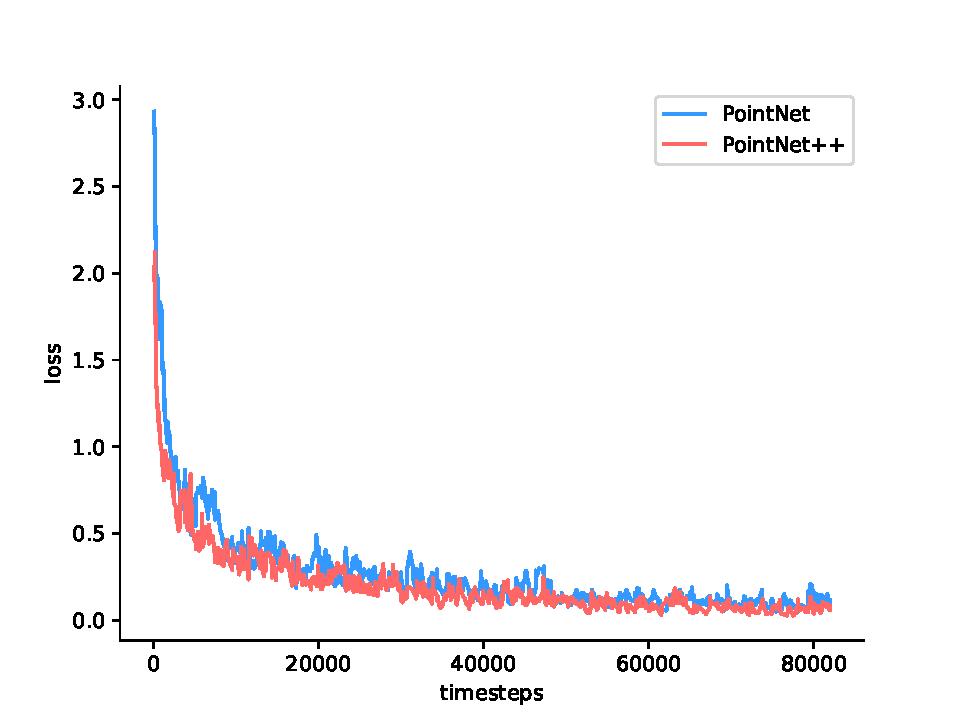
\includegraphics[width = 0.45\textwidth]{./logs/figures/pointnet_loss.pdf}
    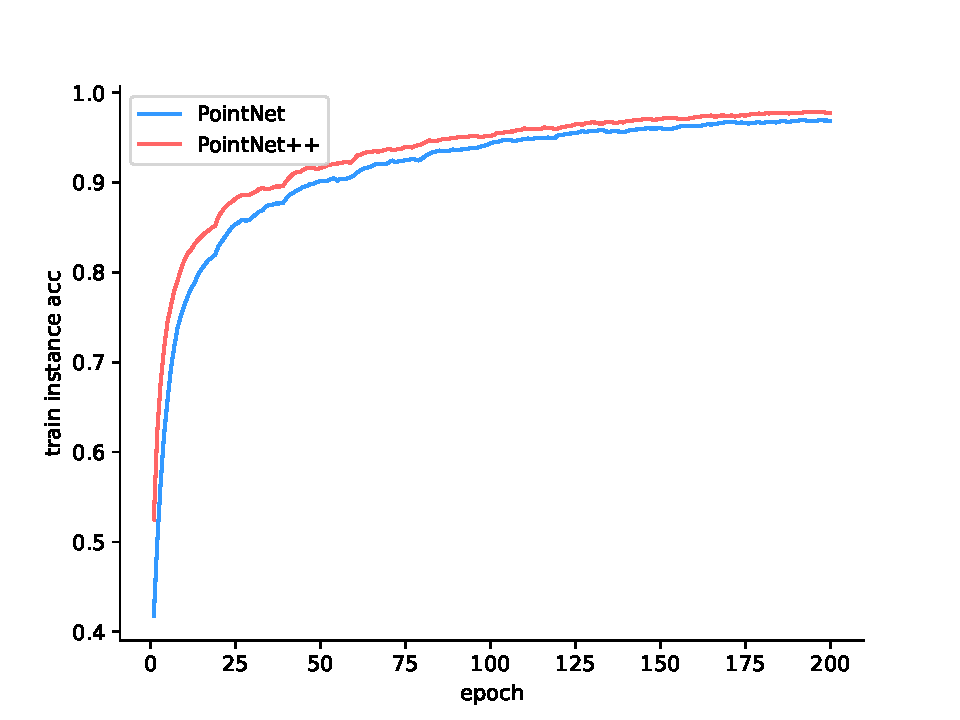
\includegraphics[width = 0.45\textwidth]{./logs/figures/pointnet_train_ins_acc.pdf}
    \caption{PointNet 和 PointNet++ 训练过程中的 Loss 和 Accuracy 曲线}
    \label{fig:pointnet_loss_acc}
\end{figure}

在测试集上两种方法的 Instance Accuracy 与 Class Accuracy 的变化曲线见 \cref{fig:pointnet_test_acc}.
\begin{figure}[htbp]
    \centering
    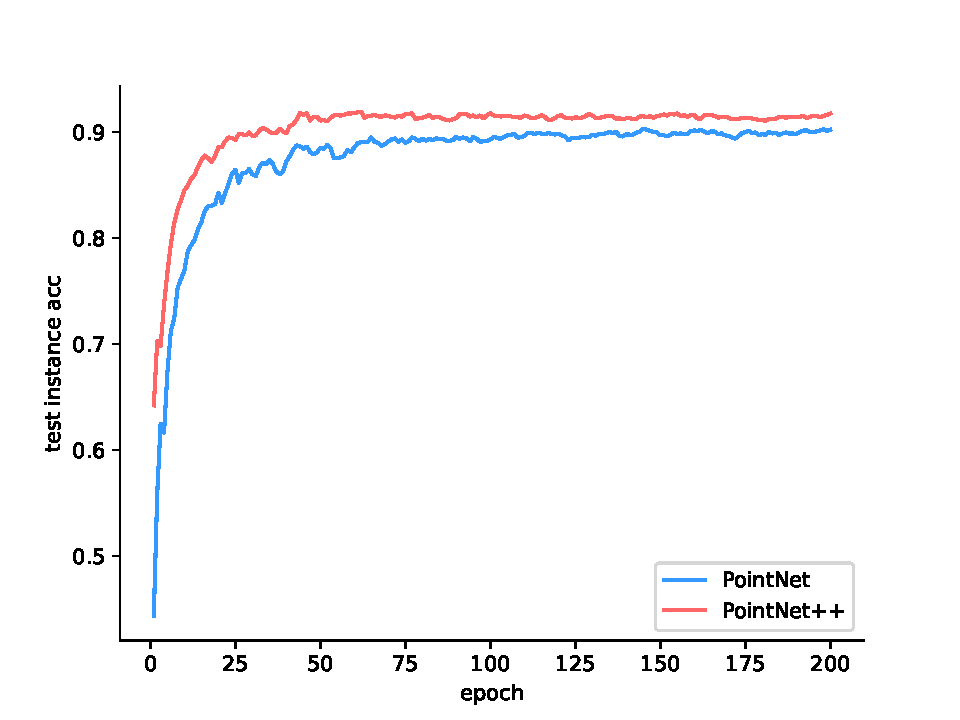
\includegraphics[width = 0.45\textwidth]{./logs/figures/pointnet_test_ins_acc.pdf}
    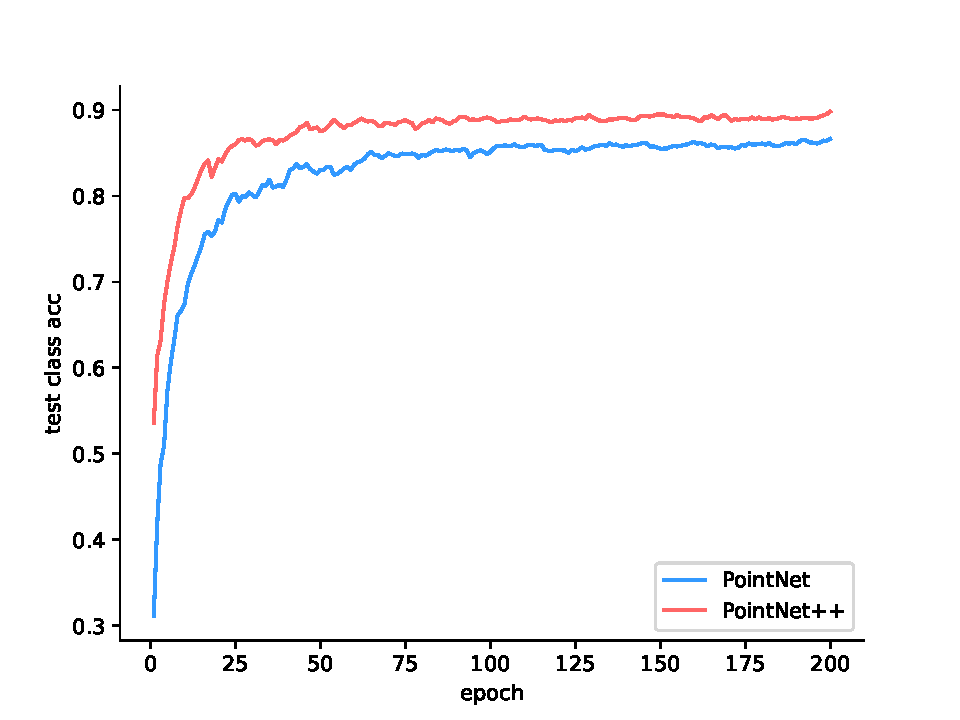
\includegraphics[width = 0.45\textwidth]{./logs/figures/pointnet_test_class_acc.pdf}
    \caption{PointNet 和 PointNet++ 测试集上的 Instance Accuracy 和 Class Accuracy 曲线}
    \label{fig:pointnet_test_acc}
\end{figure}   
与论文中汇报的结果对比见 \cref{tab:pointnet_result}. 注意 PointNet++ 使用原论文中 without normal 的结果, 
与复现的设定一致. 由于时间原因, 没有进一步复现 PointNet++ 中 使用 noraml 的结果.

\begin{table}[htbp]
    \centering
    \begin{tabular}{ccccc}
    \toprule
    & \textbf{PointNet} & \textbf{Our Result} & \textbf{PointNet++}  & \textbf{Our Result} \\
    \midrule
    Acc avg. class & 86.2 & 86.4 & N/A &  89.3\\
    Acc overall & 89.2 & 90.7 & 90.7 & 92.6\\
    \bottomrule
\end{tabular}
    \caption{在 ModelNet40 上与 PointNet 和 PointNet++ 论文中汇报的结果对比}
    \label{tab:pointnet_result}
\end{table}


\section{O-CNN}
\subsection{方法介绍}
主要的 intuition 是点云的稀疏性特点, 希望利用稀疏卷积存储稀疏的曲面信号, 把神经网络的运算限制在非空信号上以提高计算效率.

给定一个三维物体, 我们可以构造包围盒并不断相下剖分直到达到最大深度, 以此将三维物体转化为八叉树的形式. 而后利用在八叉树上定义的稀疏卷积操作和池化操作就可以构建出稀疏卷积神经网络.
通过八叉树的分层结构(每一层是 shuffle key 数组以及标记非空节点序号数组, 以此实现高速访问同父节点邻居), 可以在不同的分辨率上进行卷积操作, 并且并行化程度高, 可以在 GPU 上高效地实现.

相较于体素神经网络, O-CNN 的稀疏卷积神经网络在内存占用和计算速度上都更有优势, 同时八叉树的数据结构也可以进一步应用在 3D Transformer 中. 
\subsection{结果复现}
使用默认参数进行训练和测试, 详见\texttt{/ocnn/configs/cls\_m40.yaml}. 训练过程中的 Loss 和 Accuracy 曲线见 \cref{fig:ocnn_loss_acc}.
其中 Loss 在 120 epoch 左右骤减的原因的训练学习率使用阶梯衰减. 
\begin{figure}[htbp]
    \centering
    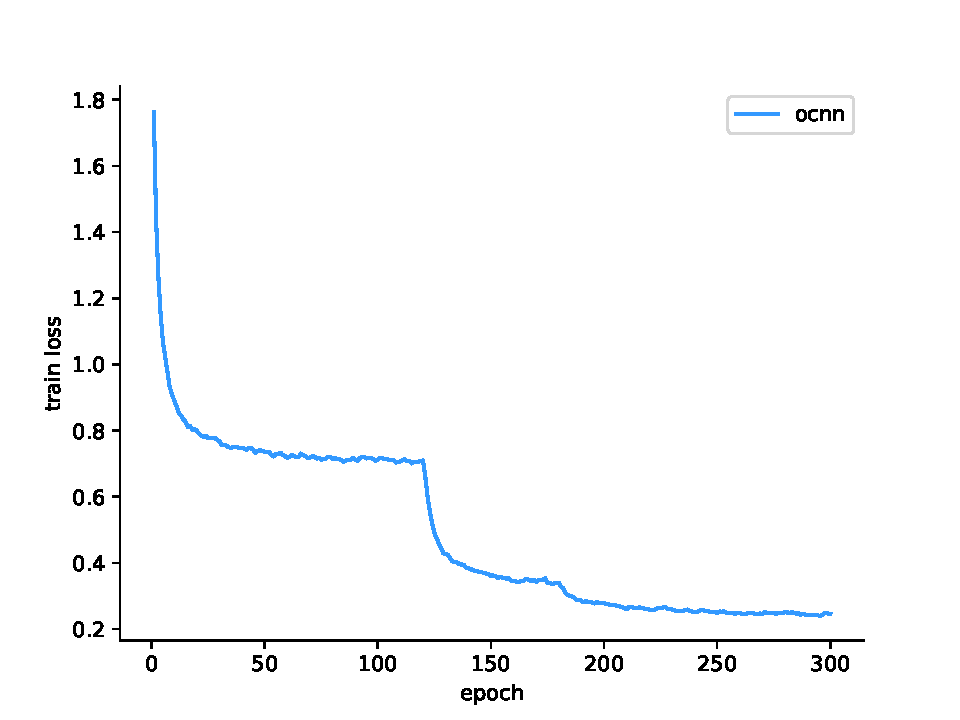
\includegraphics[width = 0.45\textwidth]{./logs/figures/ocnn_loss.pdf}
    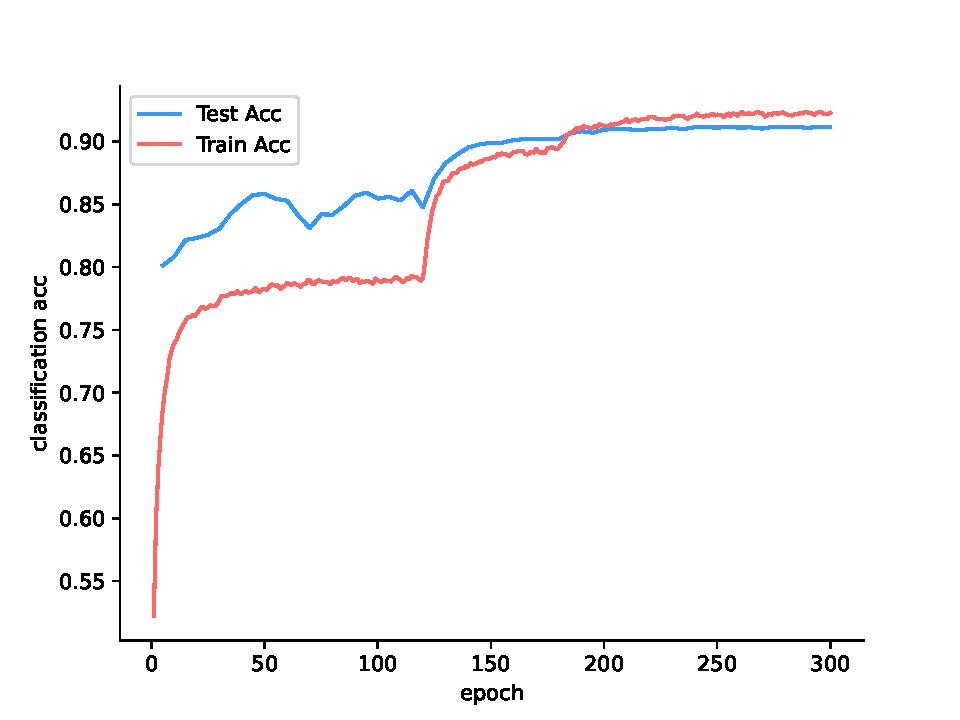
\includegraphics[width = 0.45\textwidth]{./logs/figures/ocnn_acc.pdf}
    \caption{OCNN 训练过程中的 Loss 和 Accuracy 曲线}
    \label{fig:ocnn_loss_acc}
\end{figure}

在 6 层 O-CNN without voting 的设定中, 论文汇报的结果为 89.9\%, 复现的结果为 91.5 \%.

\section{Comparison}
对于 PointNet, PointNet++ 和 O-CNN 的参数量, 分类效果与运行速度对比见 \cref{tab:compare}. 
由于不可抗的因素, PointNet 和 PointNet++ 在 4090 D 上进行训练, 而 O-CNN 在 A6000 上进行训练, 
因此运行速度的对比仅供参考. 具体分析见下: 
\begin{table}[htbp]
    \centering
    \begin{tabular}{cccccc}
    \toprule
    & \textbf{PointNet} & \textbf{PointNet++} & \textbf{O-CNN}  \\
    \midrule
    Parameters & 41.8 MB & 17.8 M & 2.4 M\\
    Accuracy(\%) & 90.7 & 92.6 & 91.5\\
    Time (s/epoch) & 68 & 42 & 24 \\
    \bottomrule
\end{tabular}
    \caption{PointNet, PointNet++ 和 O-CNN 的参数量, 分类效果与运行速度对比}
    \label{tab:compare}
\end{table}

\begin{itemize}
    \item 参数量: O-CNN 使用基于八叉树的稀疏卷积, 其参数量小于基于MLP的 PointNet 和 PointNet++. 这里汇报的参数量是保存的 \texttt{checkpoint.pth} 的文件大小. 
    \item 准确率: 在复现的结果中, O-CNN 的准确率略低于 PointNet++ 的准确率, 但高于 PointNet 的准确率. PointNet++ 是基于 PointNet 的改进, 提高了多尺度特征提取的能力, 
    如果看论文中汇报的结果, O-CNN 与 PointNet++ 的准确率相近, 但 O-CNN 的参数量更小.
    \item 运行速度: O-CNN 的运行速度快于 PointNet 和 PointNet++, 这得益于其使用的稀疏卷积, 使得其在训练时的内存占用更小, 计算速度更快.
\end{itemize}
\bibliographystyle{plain} 
\bibliography{ref} 

\end{document}